\documentclass[aspectratio=169,10pt]{beamer}

% Theme source pinned to PR #88/dca1fc4, per the leader's comment on issue #32.
% Noto Sans is required. Only the two used theme backgrounds are included.
\def\slideContentLeftMargin{0.5cm}
\def\slideContentRightMargin{0.5cm}
\def\hustHeaderHeight{1cm}
\def\slideContentTopPadding{0cm}
\IfFileExists{report/mau-slide-hust/beamerthemeHUST.sty}{
  \usepackage[blue,169]{report/mau-slide-hust/beamerthemeHUST}
}{
  \usepackage[blue,169]{mau-slide-hust/beamerthemeHUST}
}
\graphicspath{{report/mau-slide-hust/images/}{mau-slide-hust/images/}}
\useThinBar
\useStyleFull
\usefonttheme{professionalfonts}
\usepackage{fontspec}
\setmainfont{Noto Sans}
\setsansfont{Noto Sans}
\setmonofont{Noto Sans}
\usepackage{booktabs,tabularx,array}
\usepackage{tikz}
\usetikzlibrary{arrows.meta,positioning}

\definecolor{gymblue}{HTML}{174A6E}
\definecolor{gymgreen}{HTML}{317A58}
\definecolor{draftred}{HTML}{A52828}
\setbeamercolor{structure}{fg=gymblue}
\setbeamercolor{title}{fg=gymblue,bg=white}
\setbeamercolor{subtitle}{fg=black!65}
\setbeamercolor{author in head/foot}{fg=black!70,bg=black!4}
\setbeamercolor{date in head/foot}{fg=gymblue,bg=black!4}
\setbeamercolor{frametitle}{fg=white}
\setbeamercolor{block title}{fg=white,bg=gymblue}
\setbeamercolor{block body}{bg=blue!4}
\setbeamertemplate{navigation symbols}{}
\setbeamertemplate{itemize item}{\color{gymblue}\small$\blacktriangleright$}
\setbeamertemplate{itemize subitem}{\color{gymgreen}\scriptsize$\bullet$}
% Keep the theme's HUST logo visible; status/footer sits to its right.
\setbeamertemplate{footline}{%
  \hbox to \paperwidth{\hskip4.7cm%
    \normalfont\fontsize{5.5}{6.5}\selectfont\color{draftred}%
    DRAFT — chờ bộ tài liệu và kiểm chứng bàn giao\hfill%
    \color{gymblue}\insertframenumber/\inserttotalframenumber\hskip.3cm}%
  \vskip2pt%
}

\title[Bàn giao Sprint 1]{Bàn giao Sprint 1\\Web quản lý chuỗi phòng tập Gym}
\subtitle{Nhóm 6 · IT3180 · snapshot main 3ff0ae1}
\author{Nhóm 6}
\institute{Đại học Bách khoa Hà Nội}
\date{14/11/2026}

\begin{document}

% Place project text in the white area of the supplied cover background.
{
  \setbeamertemplate{background}{\includegraphics[width=\paperwidth,height=\paperheight]{\hustbg{title}}}
  \begin{frame}[plain]
    \begin{tikzpicture}[remember picture,overlay]
      \node[anchor=west,text width=.43\paperwidth,align=left,inner sep=0]
        at ([xshift=.55cm,yshift=-.1cm]current page.west) {
          {\Large\bfseries\color{hustprimary} BÀN GIAO SPRINT 1\par}
          \vspace{.3cm}
          {\large\bfseries Web quản lý chuỗi\\phòng tập Gym\par}
          \vspace{.3cm}
          {\small Nhóm 6 · IT3180\par Đại học Bách khoa Hà Nội\par 14/11/2026\par}
          \vspace{.3cm}
          {\scriptsize\color{draftred} DRAFT — chờ tài liệu và kiểm chứng bàn giao.\par}
      };
    \end{tikzpicture}
  \end{frame}
}

\begin{frame}{Snapshot bàn giao}
\small
\begin{itemize}
    \item Snapshot \texttt{main 3ff0ae1}, ngày 14/11/2026: SRS tổng quan, ERD xuất bản, từ điển, chỉ mục 31 story, schema \#101, F2 \#97, vá JWT \#105, wireframe \#78 và F4/F5 \#106, API F3 \#107 và SRS F8 \#79 đã merge.
    \item Bảng truy vết \#98 đã merge; F8 trong bảng vẫn ghim bản nháp, cần cập nhật sang F8 đã merge ngày 13/11.
    \item Backend có JWT/API auth, schema 39 bảng và F2 trên main; proxy \#99 đã đóng, không merge.
    \item Frontend F1 \#80 Ready: cục bộ 24/24 HTTP, 32/32 trình duyệt; HTTPS preview 15/15 ngày 12/11. Postman F1--F3 có kết quả của trưởng nhóm; commit backend Render còn chờ xác nhận.
  \end{itemize}
  \begin{block}{Mốc bàn giao}
    4 sprint · 20 chức năng · 6 vai trò. Sprint 1 kết thúc 09/11; demo tiếp theo 17/11/2026.
  \end{block}
  \scriptsize [\href{https://github.com/Ktin06/it3180_nhom6_gym_management/commit/3ff0ae1}{Snapshot main}] · [\href{https://github.com/Ktin06/it3180_nhom6_gym_management/actions/runs/42771961483}{CI main 872386d: success, Backend chạy, Frontend bỏ qua}]
\end{frame}

\begin{frame}{Phạm vi: 20 chức năng trong 5 version}
  \footnotesize
  \begin{tabularx}{\textwidth}{>{\bfseries\raggedright\arraybackslash}p{1.4cm} >{\raggedright\arraybackslash}X >{\raggedright\arraybackslash}p{2.6cm}}
    \toprule
    Version & Nhóm chức năng & Cam kết \\
    \midrule
    v1 & F1--F6: tài khoản, hội viên, gói, check-in, thanh toán tại quầy, dashboard & Bắt buộc \\
    v2 & F7--F10: cổng hội viên, lớp nhóm, huấn luyện viên, thông báo & Bắt buộc \\
    v3 & F11--F17: thiết bị, POS/kho, nhân sự/lương, khuyến mãi, bảo lưu, báo cáo, audit log & Mục tiêu \\
    v4 & F18--F19: đa chi nhánh, gamification theo quy tắc & Mục tiêu; cắt thứ hai nếu trễ \\
    v5 & F20: nhận diện khuôn mặt tại quầy & Cắt đầu tiên nếu trễ \\
    \bottomrule
  \end{tabularx}
  \vfill
  \begin{block}{Ưu tiên}
    Dễ kiểm thử, dễ demo các nghiệp vụ quản lý. AI chỉ có nhận diện khuôn mặt ở v5; không làm app di động hay thanh toán online.
  \end{block}
  \scriptsize Nguồn: [\href{https://github.com/Ktin06/it3180_nhom6_gym_management/blob/main/docs/requirements/ban-chot-pham-vi.md}{bản chốt phạm vi}]
\end{frame}

\begin{frame}{Sáu vai trò sử dụng hệ thống}
  \begin{columns}[T,onlytextwidth]
    \column{.49\textwidth}
      \begin{block}{Nhân viên}
        \begin{itemize}
          \item \textbf{Chủ chuỗi}: cấu hình và báo cáo toàn chuỗi.
          \item \textbf{Quản lý chi nhánh}: vận hành chi nhánh.
          \item \textbf{Lễ tân}: hồ sơ, check-in, bán và thu tiền tại quầy.
          \item \textbf{Huấn luyện viên}: lịch dạy, điểm danh và buổi PT.
        \end{itemize}
      \end{block}
    \column{.49\textwidth}
      \begin{block}{Người dùng bên ngoài}
        \begin{itemize}
          \item \textbf{Hội viên}: xem gói, đặt lớp/PT, nhận thông báo.
          \item \textbf{Khách}: xem giá, lịch lớp công khai, đăng ký.
        \end{itemize}
        Năm vai trò đăng nhập; Khách dùng trang công khai.
      \end{block}
      \begin{alertblock}{Phạm vi triển khai}
        v1--v3 dùng một chi nhánh mặc định; đa chi nhánh thuộc v4.
      \end{alertblock}
  \end{columns}
\end{frame}

\begin{frame}{Yêu cầu bảo mật và chất lượng đã chốt}
  \small
  \begin{columns}[T,onlytextwidth]
    \column{.49\textwidth}
      \begin{block}{Bảo mật}
        \begin{itemize}
          \item \textbf{S1}: bcrypt; mật khẩu từ 8 ký tự, có chữ và số.
          \item \textbf{S2}: access JWT 15 phút; refresh token trong cookie \texttt{HttpOnly}.
          \item \textbf{S3}: backend kiểm tra vai trò và quyền sở hữu trên mọi API; hội viên không xem dữ liệu người khác.
        \end{itemize}
      \end{block}
    \column{.49\textwidth}
      \begin{block}{Chất lượng}
        \begin{itemize}
          \item \textbf{NF4}: responsive từ 360 px; Chrome, Edge, Firefox bản mới.
          \item \textbf{NF6}: giao dịch có khóa bản ghi khi đặt lớp/PT; không vượt sĩ số hoặc trùng lịch dưới đồng thời.
        \end{itemize}
      \end{block}
      \begin{alertblock}{Phân biệt}
        Đây là tiêu chí đã duyệt; chưa phải kết quả nghiệm thu.
      \end{alertblock}
  \end{columns}
  \vfill
  \scriptsize Nguồn: [\href{https://github.com/Ktin06/it3180_nhom6_gym_management/blob/main/docs/requirements/ban-chot-pham-vi.md}{bản chốt phạm vi}], mục S1--S3 và NF4/NF6.
\end{frame}

\begin{frame}{Kiến trúc đích — chưa phải deployment đang chạy}
  \centering
  \begin{tikzpicture}[
    box/.style={draw=gymblue,rounded corners,fill=blue!4,minimum height=1.35cm,text width=2.55cm,align=center,font=\small},
    arr/.style={-{Latex[length=2mm]},thick,gymblue},
    node distance=0.55cm
  ]
    \node[box] (browser) {Trình duyệt\\React + Vite};
    \node[box,right=of browser] (proxy) {Proxy cùng domain\\Vite local / Vercel deploy};
    \node[box,right=of proxy] (api) {Backend\\Java 21 · Spring Boot};
    \node[box,right=of api] (db) {Cơ sở dữ liệu\\PostgreSQL};
    \draw[arr] (browser) -- node[above=20pt,font=\tiny,align=center]{\texttt{/api/v1}} (proxy);
    \draw[arr] (proxy) -- node[above=20pt,font=\tiny]{HTTP API} (api);
    \draw[arr] (api) -- node[above=20pt,font=\tiny]{JPA / Flyway} (db);
  \end{tikzpicture}
  \vspace{1em}
  \begin{alertblock}{Trạng thái hiện tại}
    Cấu hình Vercel trên main đã trỏ tới Render (\#101); \#99 đã đóng, không merge. Luồng API cùng domain đã chạy cục bộ qua proxy Vite (\#80, 24/24 HTTP). Trên staging, trưởng nhóm báo 12/11 rằng \texttt{/api/v1/auth/me} qua Vercel trả 401 đúng khi không có token; HTTPS preview của \#80 đã kiểm chứng ngày 12/11.
  \end{alertblock}
  \scriptsize Nguồn: [\href{https://github.com/Ktin06/it3180_nhom6_gym_management/blob/main/docs/decisions/0008-goi-api-cung-domain.md}{ADR 0008}] · [\href{https://github.com/Ktin06/it3180_nhom6_gym_management/blob/main/frontend/vercel.json}{cấu hình Vercel}]
\end{frame}

\begin{frame}{Dữ liệu: ERD v2 có 39 bảng, 8 nhóm}
  \small
  \begin{columns}[T,onlytextwidth]
    \column{.5\textwidth}
      \begin{enumerate}
        \item Tài khoản và hệ thống
        \item Chi nhánh và cơ sở vật chất
        \item Hội viên và gói tập
        \item Check-in và lớp học
      \end{enumerate}
    \column{.5\textwidth}
      \begin{enumerate}\setcounter{enumi}{4}
        \item Huấn luyện viên
        \item Bán hàng và thanh toán
        \item Nhân sự
        \item Gamification
      \end{enumerate}
  \end{columns}
  \begin{block}{Nguồn dữ liệu thiết kế}
    \texttt{erd-v2.dbml} là bản chuẩn; DBML Enum chỉ mô tả tập giá trị logic. CSDL vật lý dùng \texttt{varchar} + \texttt{CHECK}.
  \end{block}
  \begin{alertblock}{Báo cáo}
    PR \#96 đã merge: PDF/PNG từ dbdiagram.io, hình vector theo nhóm và từ điển 39 bảng/422 cột/89 quan hệ. Schema vật lý \#101 đã merge; trên PostgreSQL 16 cục bộ, Flyway áp 45 migration (gồm dữ liệu mẫu) và tạo 39 bảng.
  \end{alertblock}
  \scriptsize [\href{https://github.com/Ktin06/it3180_nhom6_gym_management/blob/main/docs/design/erd/erd-v2.dbml}{Mở DBML ERD v2}] · [\href{https://github.com/Ktin06/it3180_nhom6_gym_management/issues/15}{Issue \#15}]
\end{frame}


\begin{frame}{ERD đã xuất bản — nhóm hội viên và gói tập}
  \centering
  \IfFileExists{docs/design/erd/hinh/nhom-3.pdf}{
    \includegraphics[height=5.8cm]{docs/design/erd/hinh/nhom-3.pdf}
  }{
    \includegraphics[height=5.8cm]{../docs/design/erd/hinh/nhom-3.pdf}
  }
  \par\scriptsize Hình vector đã duyệt trong PR \#96, sinh từ DBML chuẩn; bảng xám là tham chiếu ngoài nhóm.\par
  [\href{https://github.com/Ktin06/it3180_nhom6_gym_management/blob/main/docs/design/erd/xuat-ban-erd.md}{Tổng quan và tám nhóm ERD}] · [\href{https://github.com/Ktin06/it3180_nhom6_gym_management/blob/main/docs/design/erd/tu-dien-du-lieu.md}{Từ điển dữ liệu}]
\end{frame}

\begin{frame}{Địa chỉ staging và kiểm tra truy cập}
  \begin{itemize}
    \item Frontend: \href{https://it3180-nhom6-gym.vercel.app}{it3180-nhom6-gym.vercel.app}.
    \item Backend: \href{https://it3180-nhom6-gym-management.onrender.com}{Render — Gym Management}.
    \item Ngày 12/11: HTTPS trên preview nhánh \#80 tới Render đạt 15/15; cookie có HttpOnly và Secure. Postman F1--F3 có kết quả của trưởng nhóm ở \#31.
    \item Render Free có thể khởi động chậm. Không suy ra backend chết từ timeout; không chạy công cụ giữ thức định kỳ.
  \end{itemize}
  \begin{alertblock}{Chưa phải demo tích hợp hoàn chỉnh}
    Có URL không đồng nghĩa API/cookie hoạt động. Schema \#101, F2 \#97 và F3 \#107 đã merge; preview HTTPS của \#80 đã chạy; mã commit backend còn chờ Tiến/Đức Việt xác nhận.
  \end{alertblock}
  \scriptsize [\href{https://github.com/Ktin06/it3180_nhom6_gym_management/issues/31\#issuecomment-6653959733}{Nguồn URL: trưởng nhóm công bố 05/11}]
\end{frame}

\begin{frame}{Sơ đồ nghiệp vụ có trong \texttt{main}}
  \begin{columns}[T,onlytextwidth]
    \column{.49\textwidth}
      \begin{block}{Use case}
        Sơ đồ tổng quát và 6 phân rã theo actor: Chủ chuỗi, Quản lý chi nhánh, Lễ tân, Huấn luyện viên, Hội viên, Khách.\\[.5em]
        PR \href{https://github.com/Ktin06/it3180_nhom6_gym_management/pull/38}{\#38} đã merge.
      \end{block}
    \column{.49\textwidth}
      \begin{block}{Activity}
        Check-in tại quầy · tự động xử lý waitlist · đặt lịch PT.\\[.5em]
        PR \href{https://github.com/Ktin06/it3180_nhom6_gym_management/pull/41}{\#41} đã merge.
      \end{block}
  \end{columns}
  \begin{block}{SRS đang có trên snapshot}
    SRS tổng quan \#95 và SRS F1--F10 đã có trên main. F8 \#79 merge ngày 13/11 tại \texttt{3ff0ae1}: 9 UC, 80 bộ Given/When/Then. Bảng truy vết còn ghim F8 cũ; ADR/ERD đồng bộ ở \#109, chưa merge.
  \end{block}
  \scriptsize [\href{https://github.com/Ktin06/it3180_nhom6_gym_management/tree/main/docs/design/use-case}{Use case}] · [\href{https://github.com/Ktin06/it3180_nhom6_gym_management/tree/main/docs/design/activity}{Activity}] · [\href{https://github.com/Ktin06/it3180_nhom6_gym_management/pull/79}{PR \#79 F8}]
\end{frame}

\begin{frame}{Đăng ký hội viên — wireframe, PR \#78 đã merge}
  \begin{columns}[T,onlytextwidth]
    \column{.30\textwidth}
      \centering
      % Minh họa rút gọn bằng mã TikZ; sơ đồ chuẩn ở PR #78.
      \begin{tikzpicture}[x=1cm,y=1cm,font=\tiny]
        \draw[rounded corners,fill=black!2] (0,0) rectangle (3.5,6.3);
        \node[font=\scriptsize\bfseries] at (1.75,5.95) {Tạo tài khoản hội viên};
        \node[align=center] at (1.75,5.55) {Chi nhánh mặc định\\Chưa bao gồm mua gói tập};
        \foreach \label/\y in {Họ và tên */4.9,Email */4.25,Số điện thoại */3.6,Mật khẩu */2.95,Xác nhận mật khẩu */2.3,Ngày sinh (tùy chọn)/1.65,Giới tính (tùy chọn)/1.0} {
          \node[anchor=west] at (.2,\y+.17) {\label};
          \draw[fill=white,draw=black!35] (.2,\y-.18) rectangle (3.3,\y+.02);
        }
        \draw[fill=gymblue,draw=gymblue,rounded corners] (.2,.25) rectangle (3.3,.58);
        \node[text=white] at (1.75,.415) {Đăng ký};
        \node at (1.75,.08) {Đã có tài khoản? Đăng nhập};
      \end{tikzpicture}
    \column{.66\textwidth}
      \begin{itemize}
        \item Bố cục tham chiếu mobile 360 px; bản chuẩn là \texttt{.drawio.svg} chỉnh sửa được.
        \item Họ tên, email, SĐT, mật khẩu; không cho tự chọn role hoặc chi nhánh.
        \item SĐT đã có hồ sơ: từ chối và hướng dẫn liên hệ quầy, không tự gắn tài khoản.
        \item Đăng ký tài khoản chưa phải mua hay kích hoạt gói tập.
      \end{itemize}
      \vspace{1em}
      \small Hình TikZ rút gọn để trình chiếu; không thay wireframe chỉnh sửa được và không phải UI đang chạy.
      \vspace{1em}

      \scriptsize [\href{https://github.com/Ktin06/it3180_nhom6_gym_management/pull/78}{PR \#78: đăng ký, bảng giá, lịch lớp}]\\
      Đã merge 10/11 tại \texttt{896c1aa}. Wireframe F4/F5 của Lân đã vào main qua \#106, không còn trong diff \#78.
  \end{columns}
\end{frame}

\begin{frame}{Lịch lớp công khai — wireframe, PR \#78 đã merge}
  \centering
  % Các tên lớp/giờ chỉ minh họa cấu trúc từ PR #78.
  \begin{tikzpicture}[x=1cm,y=1cm,font=\scriptsize]
    \draw[fill=black!2,rounded corners] (0,0) rectangle (13.8,3.9);
    \node[anchor=west,font=\small\bfseries] at (.2,3.6) {Lịch lớp học nhóm};
    \node[anchor=west] at (.2,3.15) {< Tuần trước \qquad [Ngày đầu] -- [Ngày cuối] \qquad Tuần sau >};
    \node[anchor=east] at (13.5,3.15) {Loại lớp: Tất cả};
    \foreach \day/\x in {Thứ Hai/0,Thứ Ba/1,Thứ Tư/2,Thứ Năm/3,Thứ Sáu/4,Thứ Bảy/5,Chủ nhật/6} {
      \draw[draw=black!30,fill=white] (.2+\x*1.92,.35) rectangle (2.12+\x*1.92,2.7);
      \node[align=center] at (1.16+\x*1.92,2.4) {\day\\{[dd/mm]}};
    }
    \foreach \title/\time/\state/\x in {Yoga/18:00--19:00/Theo lịch/0,Zumba/17:30--18:30/Đã đổi giờ/2,Boxing/18:00--19:00/Đã hủy/4} {
      \node[font=\tiny,align=center,fill=blue!5,inner sep=3pt,text width=1.65cm] at (1.16+\x*1.92,1.25) {\textbf{\title}\\\time\\{[Phòng]}\\{[PT phụ trách]}\\\state};
    }
  \end{tikzpicture}
  \par\vspace{.4em}
  \small Khách xem lịch không cần tài khoản. Đặt lớp cần TIME ACTIVE hợp lệ; không công khai danh sách hội viên.\par
  \vspace{.4em}
  \scriptsize Minh họa TikZ rút gọn theo sơ đồ commit \texttt{464a31a}; tên lớp/giờ là dữ liệu mẫu, không phải lịch vận hành thật.\par
  [\href{https://github.com/Ktin06/it3180_nhom6_gym_management/pull/78}{PR \#78 đã merge}] · Dashboard đã merge ở [\href{https://github.com/Ktin06/it3180_nhom6_gym_management/pull/42}{PR \#42}].
\end{frame}

\begin{frame}{Trạng thái mã nguồn và tích hợp}
\small
\begin{columns}[T,onlytextwidth]
    \column{.49\textwidth}
      \begin{block}{Frontend}
        Main còn công cụ giả lập role cho phát triển. PR \#80 bổ sung đăng ký, xác thực và menu theo role, kèm phục hồi phiên lỗi. Đã thử cục bộ với backend và CSDL thật (24/24 HTTP, 32/32 trình duyệt); HTTPS preview đạt 15/15; còn xác nhận commit Render và review.
      \end{block}
      \begin{block}{Giao diện khác}
        Wireframe F2/F3 (\#89), cổng hội viên/PT (\#102), F4/F5 (\#106) và trang công khai (\#78) đã merge. UI F2/F3 \#103 còn Draft; không trình bày như đã tích hợp backend.
      \end{block}
    \column{.49\textwidth}
      \begin{block}{Backend F1}
        JWT/phân quyền \#87 và đăng ký/login/refresh/logout \#91 đã merge. F2 \#97 đã merge: đăng ký ghi hồ sơ hội viên bền vững (kiểm chứng cục bộ). Bản vá JWT \#105 đã merge 10/11.
      \end{block}
      \begin{block}{CSDL / F2}
        Schema 39 bảng \#101 và API hồ sơ hội viên F2 \#97 đã merge. API danh mục gói F3 \#107 đã merge 11/11.
      \end{block}
  \end{columns}
  \scriptsize [\href{https://github.com/Ktin06/it3180_nhom6_gym_management/pull/80}{PR \#80}] · [\href{https://github.com/Ktin06/it3180_nhom6_gym_management/pull/97}{PR \#97}] · Snapshot \texttt{main 3ff0ae1}.
\end{frame}

\begin{frame}{Bằng chứng hiện có — và giới hạn của bằng chứng}
\small
\begin{itemize}
    \item CI \href{https://github.com/Ktin06/it3180_nhom6_gym_management/actions/runs/42771961483}{\#42771961483}: success trên \texttt{main 872386d}; job Backend (Maven, Testcontainers) chạy thật, job Frontend bỏ qua vì không đổi frontend.
    \item Frontend \#80, commit \texttt{2162417}: CI run \href{https://github.com/Ktin06/it3180_nhom6_gym_management/actions/runs/43252854032}{\#43252854032} xanh (Backend, Frontend).
    \item Tích hợp cục bộ \#80 (12/11): backend \texttt{main 336e13c} và PostgreSQL 16 thật: 24/24 HTTP, 5/5 phân quyền, 32/32 trình duyệt gồm tải lại, đăng xuất, lỗi mạng, và 360 px.
    \item HTTPS preview \#80 ngày 12/11: 15/15; đăng ký, đăng nhập, tải lại/tab mới, đăng xuất, cookie HttpOnly/Secure và 360 px. Nguồn: guide tại \texttt{2162417}.
    \item SRS tổng quan \#95, ERD/từ điển \#96 và truy vết \#98 đã merge.
  \end{itemize}
  \begin{alertblock}{Giới hạn}
    Chờ Tiến/Đức Việt xác nhận commit Render của phiên HTTPS; chưa thử lỗi mạng và vai trò nhân viên trên staging. Postman do trưởng nhóm chạy, chưa tái chạy độc lập. Chưa nghiệm thu toàn bộ NF/S.
  \end{alertblock}
\end{frame}

\begin{frame}{Phụ thuộc và rủi ro trước khi demo}
\small
  \begin{itemize}
    \item \textbf{Staging:} HTTPS preview \#80 đạt 15/15 ngày 12/11; chờ xác nhận commit backend Render theo review 13/11.
    \item \textbf{Postman F1--F3 (\#31, đã đóng):} kết quả 12/11: F1 9/11, F2 25/26, F3 31/34 kiểm tra đạt; các bước lỗi do dữ liệu staging. Chưa tái chạy độc lập.
    \item \textbf{API và bảo mật:} F3 \#107 và bản vá JWT \#105 đã merge; cần xác nhận lại trên staging.
    \item \textbf{F8 \#79:} đã merge 13/11 tại \texttt{3ff0ae1}; ADR/ERD còn ở \#109, thiết kế kỹ thuật thuộc Sprint 2.
    \item \textbf{UI \#78/\#80/\#103:} \#78 đã merge; \#80 Ready, chờ xác nhận commit Render và review; \#103 Draft.
    \item \textbf{Bàn giao:} theme HUST đã áp; còn review và rehearsal trước demo 17/11, không chờ xuất SRS/ERD.
  \end{itemize}
  \scriptsize [\href{https://github.com/Ktin06/it3180_nhom6_gym_management/issues/31}{Staging/Postman \#31}] · [\href{https://github.com/Ktin06/it3180_nhom6_gym_management/issues/32}{Bàn giao \#32}]
\end{frame}

\begin{frame}{Ma trận bàn giao — giữ nguyên người phụ trách}
\scriptsize
  \begin{tabularx}{\textwidth}{>{\bfseries\raggedright\arraybackslash}p{2.15cm} >{\raggedright\arraybackslash}X >{\raggedright\arraybackslash}p{2.55cm}}
    \toprule
    Hạng mục & Trạng thái / bước tiếp theo & Người theo phân công \\
    \midrule
    SRS / truy vết & \#95 và \#98 đã merge; F8 \#79 đã merge 13/11; truy vết cần cập nhật nguồn & Nguyễn Anh Tú; Phạm Gia Bảo (F8) \\
    ERD / dữ liệu & \#96 đã merge PDF/PNG và từ điển; schema \#101 đã merge; DBML là nguồn chuẩn & Nguyễn Anh Tú \\
    Stories / wireframe & \#77, \#78, \#102, \#106 đã merge & Gia Bảo và các chủ wireframe theo kế hoạch \\
    Schema / API & Auth, schema \#101, F2 \#97, F3 \#107 và \#105 đã merge & Chủ issue/WBS; F1 Đức Việt, F2/F3 Lân \\
    UI xác thực & \#80 Ready; HTTPS 15/15, chờ xác nhận commit Render và review & Phạm Gia Bảo \\
    Staging / Postman & Postman F1--F3 có kết quả 12/11 (theo trưởng nhóm); HTTPS preview \#80 đạt 15/15 & Phú Trọng; Kim Tiến \\
    Slide / rehearsal & Cập nhật snapshot 14/11; còn review và rehearsal & Phạm Gia Bảo \\
    \bottomrule
  \end{tabularx}
  \vfill
  \scriptsize [\href{https://github.com/Ktin06/it3180_nhom6_gym_management/blob/main/docs/plans/sprint-1-tien-do.md}{Sprint Plan}] · [\href{https://github.com/Ktin06/it3180_nhom6_gym_management/issues/31\#issuecomment-6653959733}{Xác nhận triển khai của trưởng nhóm}]. Không tự đổi phân công.
\end{frame}

\begin{frame}{Việc cần chốt trước và trong buổi trình bày 17/11}
\begin{enumerate}
    \item Tiến/Đức Việt xác nhận commit backend Render; phân biệt bản hiện hành với bản đã thử HTTPS ngày 12/11 nếu có deploy lại.
    \item Postman F1--F3 đã có kết quả ở \#31; trước demo kiểm tra lại môi trường và dữ liệu thử, nói rõ các ca thiếu dữ liệu.
    \item Tú review \#80 sau khi có commit Render; \#103 vẫn Draft, chưa nhận là tích hợp API thật. Gộp theo policy.
    \item Chủ nguồn cập nhật truy vết F8 sau \#79 đã merge; ADR/ERD tiếp tục ở \#109.
    \item Tú review slide; rehearsal với URL thật trước demo 17/11. Nếu staging không phản hồi, dùng môi trường cục bộ đã kiểm chứng và nói rõ.
  \end{enumerate}
  \vfill
  \small [\href{https://github.com/Ktin06/it3180_nhom6_gym_management/issues/31}{Staging/Postman}] · [\href{https://github.com/Ktin06/it3180_nhom6_gym_management/issues/32}{Bàn giao}] · Source-only: PDF cuối do trưởng nhóm đưa lên Release.
\end{frame}

\end{document}
